\documentclass[12pt,runningheads]{llncs}
\usepackage{graphicx}
\usepackage[
    left=3cm,
    right=3cm,
    top=4cm,
    bottom=4cm
]{geometry}
\usepackage{etoolbox}
\usepackage{array}
\apptocmd{\thebibliography}{\setlength{\itemsep}{12pt}}{}{}

\begin{document}

% Comparing the Effectiveness of Deep Learning Models
% on the Categorisation of Galaxy Morphology
\title{
    % Comparing the Effectiveness of Deep Learning Models on the Categorisation of Galaxy Morphology \\
    CMP3753M Project Proposal
}

\author{Luke Roberts}

\institute{University of Lincoln \\
\email{25722923@students.lincoln.ac.uk}}

\maketitle

\section{Introduction}
%   Overview
% - Introduce key concepts like deep learning and
%   image classification, and why they are relevent
%   to study -> What are their uses?
%
% - Introduce galaxy morphology and the importance of
%   further studying distant galaxies for bettering
%   human understanding of the cosmos -> Why is it important?
%
% - Link the two ideas and showcase previous research,
%   adding references when appropriate
%
%   Paragraph 1
% - What is deep learning and image classification
% - Image classification accurately (but not always perfectly)
%   catagorise images in a specific dataset
% - (we will be using a specific dataset of images)
% - Different image classification models work better with
%   different themed image sets
%
%   Paragraph 2
% - Astronomy and understanding the universe is important
%   for scientific research
% - Understanding galaxy forms is a small but important part
%   of astronomy
% - Because of the massive amount of data produced by
%   observatries e.g. the hubble space telescope, it takes
%   a long time for people to accurately catagorise the
%   growing dataset.
% - There exists databases of already catagorised
%   galaxies
% - We should therefore use this data to catagorise new
%   images of galaxy morphology
%
%   Conclusion
% - We should analise which Deep Learning Model is best for
%   catagorizing galaxies into different morphologies.
Understanding the universe has been a pursuit of humanity for thousands of
years. Because of the increasing effectiveness of deep learning image
classification models, categorising distant objects in space has become much
easier. Therefore, this rapid development in deep learning will allow
astrophysicists to further their research into the early universe.

Advances in observational technology such as the James Webb Space
Telescope (JWST) \cite{JWST} push the bounds of galaxy observations further
into deep space. The time taken for the light of distant galaxies to reach
us means that our night sky is a window into the past, which allows
astrophysicists to understand the evolution of our universe in more depth.
Photographs such as the Hubble Ultra-Deep field show an ancient universe full
of developing galaxies \cite{HUDF}, and the amount of observed galaxies in
astronomy databases are only increasing.

By identifying how the structure of galaxies, or galaxy morphology, changes over
time, astrophysicists have a clearer picture of changes the universe has
undergone. However, it is extremely time-consuming for astrophysicists to
categorise galaxies in their research. A study in 2016 \cite{EGND} calculated
that there are ~2.0×10¹² galaxies in the observable universe. While it would be
unnecessary to categorise every galaxy, automation accelerates research as
the distance of observations continues increasing. One powerful method for
automation of images is to train and deploy a deep learning model.

Deep Learning has recently revolutionised both scientific research and modern
life in a profound way. From automated X-ray and MRI classification;
machine translation such as Google Translate and large language models such as
ChatGPT, deep learning has become the best way to categorise, analyse and
generate unstructured data \cite{DLCTW}. To perform many of these tasks,
machine learning engineers create deep learning models which utilises a dataset
that learns patterns about that data.

Image classification is a form of deep learning that uses images as input data
and is used for a wide variety of applications in scientific research. Like
all forms of deep learning, image processing models are trained so that they
more accurately categorise new input data by analysing how the model output
differs from the expected output. All models are somewhat inaccurate but choosing
the correct model minimises error. Popular models for image classification are deep
neural networks (DNNs) and convoluted neural networks (CNNs). New deep learning
models are also being developed. One promising new model is ConvXGB which was
shown to be more acurate when compared to other deep learning models for certain
datasets \cite{CONVXGB}.

Recent studies such as (José A. de Diego et. al) \cite{GCDL} concluded that
using a DNN “outperforms” other adopted models for galaxy classification.
However, to extend this research which deep learning neural network is most
effective at classifying the morphology of distant galaxies will be evaluated.

\section{Aims and Objectives}

\subsection{Aim}
The aim of this project is to train and test deep learning models in order to
determine which is more suitable to classify the morphology of galaxies from
astronomy databases. The project will compare DNN, CNN and ConvXGB models.
Each model will be implemented in python using machine learning libraries and
trained on GPU accelerated hardware.

\subsection{Objectives}

\begin{enumerate}
    \item Collect a dataset of galaxy images, coupled with their morphological
    type using ESA astronomy archives \cite{ESAHSA} with the astropy library
    \cite{ASTROPY}.

    \item Analyse the formatting and structure of the dataset images so that
    preprocessing can be implemented.

    \item Implement image preprocessing for training in python through an image
    processing library called Pillow \cite{PIL} to training images. The rest of
    the dataset will also need to be cleaned before training.

    \item Implement deep learning models (DNN, CNN, ConvXGB) for predicting the
    categorisation of images of galaxies. The real type of morphology
    associated with that image will be used in backpropergation the of the model
    to train it. The model implementations will be built using the python
    libraries Sci-kit Learn \cite{SCIKIT}, TensorFlow \cite{TFLOW} and XGBoost
    \cite{XGB}.

    \item Deploy on hardware and train the models with the training dataset.
    Models will be tested and performance heuristics will determine which model
    is better at categorising galaxy morphology.
\end{enumerate}

\section{Project Plan and Risk Analysis}

\subsection{Project Plan}

Practical implementations and dissertation writing will be worked on
concurrently. Each stage of the implementation will be done in the order stated
above in Objectives and an appropriate amount of time is given to each task
depending on the complexity.

\begin{figure}
    \centering
    \caption{Gant Chart of project}\label{tab1}
    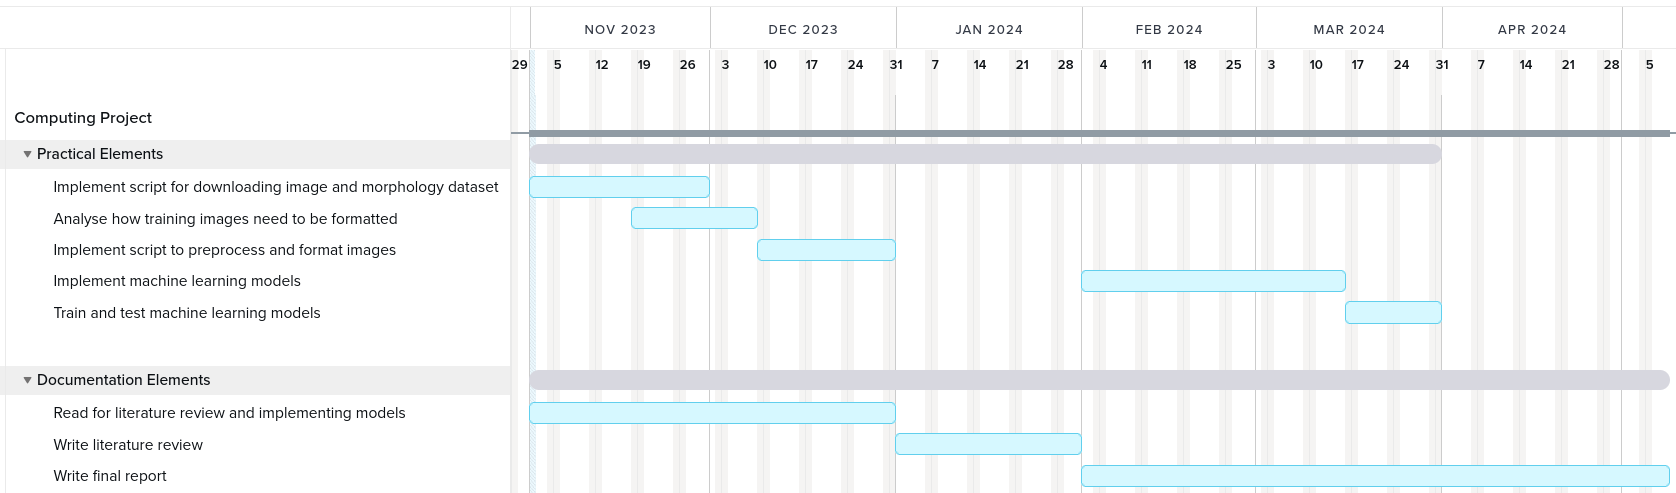
\includegraphics[width=\textwidth,scale=1.5]{GantChart.png}
\end{figure}

\newpage

\subsection{Risk Analysis}

\begin{table}
    \centering
    \caption{Table of risks, their impacts and mitigations.}\label{tab1}
    \begin{tabular}{|p{2cm}|p{2cm}|p{2cm}|p{4.5cm}|p{4.5cm}|}

        \hline
        Risk & Occurance & Impact & Explenation & Mitigation\\
        \hline
        Missing Values & Very Likely & Low & Often, databases have missing values, which either affect model performance or prevent model training entirely. & Depending on the needs of the model, any rows of the dataset that have missing values could be removed or imputed.\\
        \hline
        Biassed Dataset & Very Likely & Medium - Low & Datasets sometimes overrepresent certain classifications or clusters of data, known as bias. This means the model is trained with biassed data which when tested, leads to biassed output. & Several techniques can be used to reduce bias. Resampling can be used to artificially overrepresent smaller classes and underrepresent larger classes. Applying data transformations can also reduce bias.\\
        \hline
        Performance Issues & Likely & High & Depending on the complexity of a machine or deep learning model, the computational resources needed to train the model may be quite high. This is especially true for neural network based models that require matrix multiplication and backpropagation calculations which are expensive for processors and memory. & GPU parallelisation will be necessary in order to train the models in a much shorter amount of time. The deep learning models will then be trained on a high-end GPU.\\
        \hline
        External Database Unavailable & Unlikely & High & If external databases used for training the model are either extremely slow or unavailable, data preprocessing and training models will not be available. & The database being down will be investigated to ascertain when it will be available again. If it remains down or will be down for a longer duration, alternative databases will be used instead.\\
        \hline
    \end{tabular}
\end{table}

\newpage

\begin{thebibliography}{20}

\bibitem{JWST}
NASA (2019). Key Facts - Webb/NASA. [online] Nasa.gov. Available at:\\
https://jwst.nasa.gov/content/about/faqs/facts.html.

\bibitem{HUDF}
Hyperwall, Nasa. (2018). Hyperwall: Hubble Ultra Deep Field.
[online] svs.gsfc.nasa.gov. [online] Available at:
https://svs.gsfc.nasa.gov/30946.

\bibitem{EGND}
Conselice, C.J., Wilkinson, A., Duncan, K. and Mortlock, A. (2016). The
Evolution of Galaxy Number Density at $z < 8$ and
its Implications. The Astrophysical Journal, [online] Available at:
https://doi.org/10.3847/0004-637X/830/2/83.

\bibitem{DLCTW}
Singh, A. (2023). The Power of Deep Learning: How It's Changing the World.
[online] Medium. Available at:
https://medium.com/@Ambarish\_224/the-power-of-deep-learning-how-its-changing-the-world-13780515be31.

\bibitem{UIQDNN}
Dodge, S. and Karam, L. (2016). Understanding how image quality affects deep
neural networks. 2016 Eighth International Conference on Quality of Multimedia
Experience (QoMEX). [online] Available at:
https://doi.org/10.1109/qomex.2016.7498955.

\bibitem{CONVXGB}
Thongsuwan, S., Jaiyen, S., Padcharoen, A. and Agarwal, P. (2021). ConvXGB: A
new deep learning model for classification problems based on CNN and XGBoost.
Nuclear Engineering and Technology, tables 5a-c. [online] Available at:
https://doi.org/10.1016/j.net.2020.04.008.

\bibitem{GCDL}
Diego, J.A. de, Nadolny, J., Bongiovanni, Á., Cepa, J., Pović, M., García,
A.M.P., Torres, C.P.P., Lara-López, M.A., Cerviño, M., Martínez, R.P., Alfaro,
E.J., Castañeda, H.O., Fernández-Lorenzo, M., Gallego, J., González, J.J.,
González-Serrano, J.I., Pintos-Castro, I., Sánchez-Portal, M., Cedrés, B. and
González-Otero, M. (2020). Galaxy classification: deep learning on the OTELO and
COSMOS databases. Astronomy \& Astrophysics, [online] Accessed at:
https://doi.org/10.1051/0004-6361/202037697.

\bibitem{ESAHSA}
hst.esac.esa.int. (n.d.). ESA Hubble Science Archive. [online] Available at:\\
https://hst.esac.esa.int/ehst/\#/pages/search.

\bibitem{ASTROPY}
www.astropy.org. (n.d.). Astropy. [online] Available at:
https://www.astropy.org/.

\bibitem{PIL}
Readthedocs.io. (2011). Pillow (PIL Fork) 6.2.1 documentation. [online]\\
Available at: https://pillow.readthedocs.io/en/stable/.

\bibitem{SCIKIT}
Scikit-learn (2019). scikit-learn: machine learning in Python — scikit-learn
0.20.3 documentation. [online] Scikit-learn.org. Available at:
https://scikit-learn.org/stable/index.html.

\bibitem{TFLOW}
Google (2019). TensorFlow. [online] TensorFlow. Available at:
https://www.tensorflow.org/.

\bibitem{XGB}
xgboost.readthedocs.io. (n.d.). XGBoost Documentation — xgboost 1.7.2
documentation. [online] Available at:
https://xgboost.readthedocs.io/en/stable/\#.

\end{thebibliography}

\end{document}